\section{Lezione 2 - 07/03/2024}

% https://it.wikipedia.org/wiki/Decadimento_esponenziale
% Krane - Cap 6.3 pag 161/165
% Napolitano - Cap 1.3.1 pag 28/32

Protoni e neutroni devono essere trattenuti nel nucleo da una forza di natura diversa rispetto a quelle fino ad ora incontrate, ovvero la \textit{forza gravitazionale} e la \textit{forza elettromagnetica}. Poiché i protoni hanno carica positiva, tra di essi agisce una forza elettrostatica repulsiva. Affinché il nucleo possa rimanere stabile come un sistema legato, è necessaria un'altra forza attrattiva, più intensa della forza elettrostatica. Questa forza deve avere un raggio d'azione molto limitato, certamente più piccolo delle distanze atomiche, poiché non ha alcun effetto a tali scale. 

Nella fisica nucleare e subnucleare, le informazioni sperimentali sulla struttura di nuclei e particelle, sulle loro proprietà e sulle forze che esercitano tra loro derivano dallo studio di tre processi fondamentali: 
    \begin{enumerate}
        \item \textbf{Stati legati}: Uno stato legato è un sistema composto di due o più particelle, soggette a un potenziale interno, caratterizzato dall'avere un'energia meccanica totale $E$ negativa. Studiare queste configurazioni ci può dare informazioni importanti sulle forze che li tiene insieme.
        \item \textbf{Decadimenti}: Il decadimento è il processo di disintegrazione in cui un nucleo instabile $a$, caratterizzato dall'avere un tempo di vita finito, si trasforma spontaneamente in altri più stabili $b, c, \dots$ . Questo processo è governato da una forza specifica. Analizzandolo, possiamo identificarne l'origine. 
        \item \textbf{Collisioni}: Le collisioni tra particelle sono urti in cui una o più particelle proiettile $a$ interagiscono in vari modi con una o più particelle bersaglio $b$. Tali interazioni possono portare alla formazione di diversi prodotti, in base al tipo di interazione in gioco. Poiché queste interazioni sono mediate da una o più forze, il loro studio ci aiuta a caratterizzarle.
    \end{enumerate}
Tutti e tre questi processi avvengono in accordo con dei principi di conservazione universali: energia, quantità di moto, momento angolare e carica. Questi principi di conservazione vengono sempre rispettati, indipendetemente dal tipo di processo in esame. 

Per le leggi di conservazione, quando un nucleo decade è richiesto che i prodotti siano almeno due particelle e/o nuclei. 

I processi di collisione si dividono in due tipi:
    \begin{itemize}
        \item \textit{Urti elastici}: Una collisione nella quale le particelle nello stato finale sono le stesse di quello iniziale.
            \begin{equation*}
                a + b \to a + b
            \end{equation*}
        \item \textit{Urti anaelastici}: Una collisione nella quale le particelle nello stato funale sono diverse in numero e/o tipo da quelle iniziali.
            \begin{equation*}
                a + b \to c + d + f
            \end{equation*}
    \end{itemize}
Essendo che i processi di collisione tra particelle cadono nella maggioranza dei casi nel framework della fisica relativistica, le leggi di conservazione vanno intese rispetto alle grandezze fisiche relativistiche in gioco. Fissato un sistema di riferimento inerziale $O$ e data una particella con massa a riposo $m_0$, misurata nel sistema di riferimento solidale alla particella stessa, l'energia e l'impulso relativistici sono definiti dalle seguenti relazioni
    \begin{align}
        E & = m_0 c^2 + T = \gamma m_0 c^2 
        \label{eq: relativistic energy} \\
        \mathbf{p} & = \gamma m_0 \mathbf{v} 
        \label{eq: relativistic momentum}
    \end{align}
con $T = (\gamma - 1) m_0 c^2$ l'energia cinetica relativistica della particella, con $\mathbf{v}$ la velocità della particella misurata rispetto al sistema di riferimento inerziale $O$ e con $\gamma$ il \textit{fattore di Lorentz}, definito come     
    \begin{equation*}
        \gamma = \frac{1}{\sqrt{1 - \beta^2}} \quad \text{con} \quad \beta = \frac{v}{c}
    \end{equation*}
A partire dalla \eqref{eq: relativistic energy} e dalla \eqref{eq: relativistic momentum} possiamo ricavare la famosa relazione di Einstein. Partiamo da quella sull'energia
    \begin{align*}
        E & = \gamma m_0 c^2 \\
        E & = \frac{m_0 c^2}{\sqrt{1 - \beta^2}}  \\
        E^2 & = \frac{m_0^2 c^4}{1 - \beta^2} \quad \to \quad  E^2 - E^2 \beta^2 = m_0^2 c^4
    \end{align*}
Per la \eqref{eq: relativistic momentum} consideriamo invece solo il modulo
    \begin{align*}
        p & = \gamma m_0 v \\
        p c & = \gamma m_0 v c \\
        p c & = \gamma m_0 \frac{v}{c} c^2 \\
        p c & = \beta \gamma m_0 c^2 \\
        p c & = \beta E \quad \to \quad  p^2 c^2 = \beta^2 E^2
    \end{align*}
Sostituendo la relazione appena trovata all'interno di quella per l'energia troviamo
    \begin{equation*}
        E^2 = p^2 c^2 + m_0^2 c^4
    \end{equation*}
Come vedremo, la relatività ristretta estende i concetti fondanti della meccanica newtoniana. Pertanto ci possiamo aspettare che la tali relazioni si riducano a quelle della meccanica newtoniana per basse velocità. Per farlo possiamo approssimare $\gamma(\beta)$ per $\beta \ll 1$
    \begin{equation*}
        \gamma(\beta) \approx 1 + \frac{\beta^2}{2}
    \end{equation*}
avendo usando la seguente espansione in serie
    \begin{equation*}
        (1 + x)^\alpha \approx 1 + \alpha x 
    \end{equation*}
con $\alpha = -\frac{1}{2}$ e $x = -\beta^2$. Applicando questa approssimazione all'energia cinetica relativistica $T$ infatti vediamo subito come questa si riduca a quella classica
    \begin{align*}
        T = (\gamma - 1) m_0 c^2 \quad \to \quad T & = (1 + \frac{\beta^2}{2} - 1) m_0 c^2 \\
        & = \frac{\beta^2}{2} m_0 c^2 \\
        & = \frac{1}{2} m_0 \frac{v^2}{c^2} c^2 \quad \to \quad T = \frac{1}{2} m_0 v^2
    \end{align*}

\subsection{Decadimenti}
Se ho un campione di $N_0$ particelle instabili al tempo $t = 0$ e se non vengono introdotti nuovi nuclei all'interno del campione, si vede sperimentalmente che il tasso di decrescita $\lambda$, definito come il rapporto tra la variazione del numero di particelle nel tempo e il numero di particelle, non dipende dal tempo.
    \begin{equation}
        \frac{\displaystyle - \frac{d N(t)}{dt}}{N(t)} = \lambda
        \label{eq: empirical evidence decay}
    \end{equation}
La costante $\lambda$ è anche nota \textit{costante di decadimento} e ha le dimensioni dell'inverso di un tempo. Per integrazione della \eqref{eq: empirical evidence decay} otteniamo la \textit{legge del decadimento esponenziale}
    \begin{equation*}
        \boxed{N(t) = N_0 e^{- \lambda t}}
    \end{equation*}
Analogia per il caso in cui $\tau_2 \ll \tau_1$ e $\tau_1 \ll \tau_2$ 
    \begin{enumerate}
        \item $\tau_2 \ll \tau_1$: Consideriamo una situazione in cui abbiamo questo processo. Ho due tessere del domino indicate con A e B. Quando A cade allora potrà cadere anche B e quando anche B sarà caduta potrò andare a dormire, ma il tempo necessario a far cadere A e B è diverso. In questa situazione abbiamo che la tessera A cade dopo 1 secondo mentre la tessera B dopo un'ora. Durante tutto il processo quando cade A importa poco, perché essendo caduta subito dovrò per forza aspettare B prima di andare a dormire. Questo si traduce nel decadimento con il fatto che $N_2$ decade con la sua costante di tempo fregandosene di quella del genitore $N_1$.
        \item $\tau_1 \ll \tau_2$: Consideriamo una situazione in cui abbiamo questo processo. Ho due tessere del domino indicate con A e B. Quando A cade allora potrà cadere anche B e quando anche B sarà caduta potrò andare a dormire, ma il tempo necessario a far cadere A e B è diverso. In questa situazione abbiamo che la tessera A cade dopo 1 ora secondo mentre la tessera B dopo un secondo. Quando vedrò cadere A cadrà subito anche B, anche se dopo un secondo. Ma dato che ho dovuto aspettare un'ora per vedere cadere A per B cade praticamente insieme ad A. Questo si traduce nel decadimento con il fatto che $N_2$ decade con la costante di tempo del genitore perché tanto appena decade il padre, nei tempi di osservazioni tali da poter vedere il decaidmento del genitore il figlio decade praticemente immediatamente dopo.
    \end{enumerate}

    \begin{figure}[ht]
        \centering
        \begin{tikzpicture}[scale = 1, domain = 0:3.8, samples = 100]
            % \draw[style = help lines] (-1,-1) grid (4,2);
            \clip (-1,-1) rectangle (4,2);

            \draw[->] (0,-0.5) -- (0,2) node[below left] {$N(t)$};
            \draw[->] (-0.5,0) -- (3.9,0) node[below] {$t$};

            \draw[thick] plot(\x, {exp(-\x)});
        \end{tikzpicture}
        \caption{Decadimento esponenziale del numero di nuclei instabili.}
        \label{fig: Exponential decay}
    \end{figure}

    \begin{figure}[ht]
        \centering
        \begin{tikzpicture}[scale = 1, domain = 0:3.8, samples = 100]
            % \draw[style = help lines] (-1,-1) grid (4,2);
            \clip (-1,-1) rectangle (4,2);

            \draw[->] (0,-0.5) -- (0,2) node[below left] {$N_2(t)$};
            \draw[->] (-0.5,0) -- (3.9,0) node[below] {$t$};

            \draw[thick] plot(\x, {2*exp(-\x) - 2*exp(-5*\x)});
        \end{tikzpicture}
        \caption{Decadimento esponenziale del numero di nuclei figli in un decadimento a cascata.}
        \label{fig: Exponential decay chain}
    \end{figure}

    \begin{figure}[ht]
        \centering
        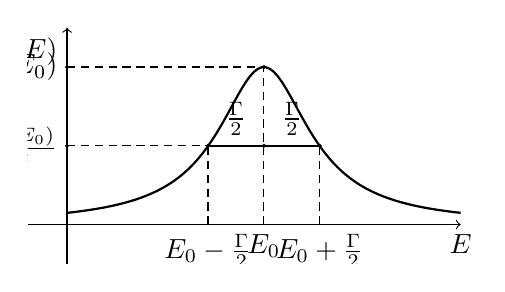
\begin{tikzpicture}[scale = 1, domain = 0:5, samples = 100]
            % \draw[style = help lines] (-0.5,-0.5) grid (5.2,2.5);
            \clip (-0.5,-0.5) rectangle (5.2,2.5);

            \draw[->] (0,-0.5) -- (0,2.5) node[below left] {$P(E)$};
            \draw[->] (-0.5,0) -- (5,0) node[below] {$E$};

            \draw[densely dashed] (2.5, 0) node[below] {$E_0$} -- (2.5, 2);
            \draw[densely dashed] (3.21, 0) node[below] {$E_0 + \frac{\Gamma}{2}$} -- (3.21, 1);
            \draw[densely dashed] (1.79, 0) node[below] {$E_0 - \frac{\Gamma}{2}$} -- (1.79, 1);

            \draw[thick] (1.79, 1) -- node[above] {$\frac{\Gamma}{2}$} (2.5, 1);
            \draw[thick] (2.5, 1) -- node[above] {$\frac{\Gamma}{2}$} (3.21, 1);

            \draw[densely dashed] (0, 2) node[left] {$P(E_0)$} -- (2.5, 2);
            \draw[densely dashed] (0,1) node[left] {$\frac{P(E_0)}{2}$} -- (3.21, 1);

            \filldraw[] (2.5, 2) circle (0.5pt);
            \filldraw[] (2.5, 1) circle (0.5pt);
            \filldraw[] (3.21, 1) circle (0.5pt);
            \filldraw[] (1.79, 1) circle (0.5pt);
            \filldraw[] (0, 2) circle (0.5pt);
            \filldraw[] (0, 1) circle (0.5pt);

            \draw[thick] plot(\x, {1/((\x-2.5)^2 + 0.5)});
        \end{tikzpicture}
        \caption{Distribuzione Breit-Wigner}
        \label{fig: Breit-Wigner}
    \end{figure}